\documentclass{article}
\usepackage[margin=1in]{geometry}
\usepackage{amsmath}
\usepackage{amssymb}
\usepackage{amsthm}
\usepackage{bm}
\usepackage{hyperref}
\usepackage{graphicx}
\usepackage{caption}
\usepackage{listings}
\usepackage{xcolor}
\usepackage{float}
\usepackage{booktabs}
\usepackage{longtable}
\usepackage{multirow}
\usepackage{placeins}
\graphicspath{{figures/}}

% Code style
\lstdefinestyle{code}{
  basicstyle=\ttfamily\small,
  numbers=left,
  numberstyle=\tiny,
  numbersep=8pt,
  keywordstyle=\color{blue},
  commentstyle=\color{teal!70!black},
  stringstyle=\color{orange!70!black},
  showstringspaces=false,
  breaklines=true,
  frame=single,
  framerule=0.3pt,
  rulecolor=\color{black!15}
}
\lstset{style=code}

\title{Compression and Distillation: Pruning, Quantization, and TinyLLM Edge Deployment}
\author{}
\date{\today}

\begin{document}
\maketitle

\section{Pruning and Quantization}
\subsection{Compression roadmap}
Figure~\ref{fig:compression_landscape_en} outlines a typical path from dense LLMs to compact deployable models: pruning removes redundant structure, quantization reduces numeric precision, and distillation produces student models tailored for constrained devices.
\begin{figure}[H]
  \centering
  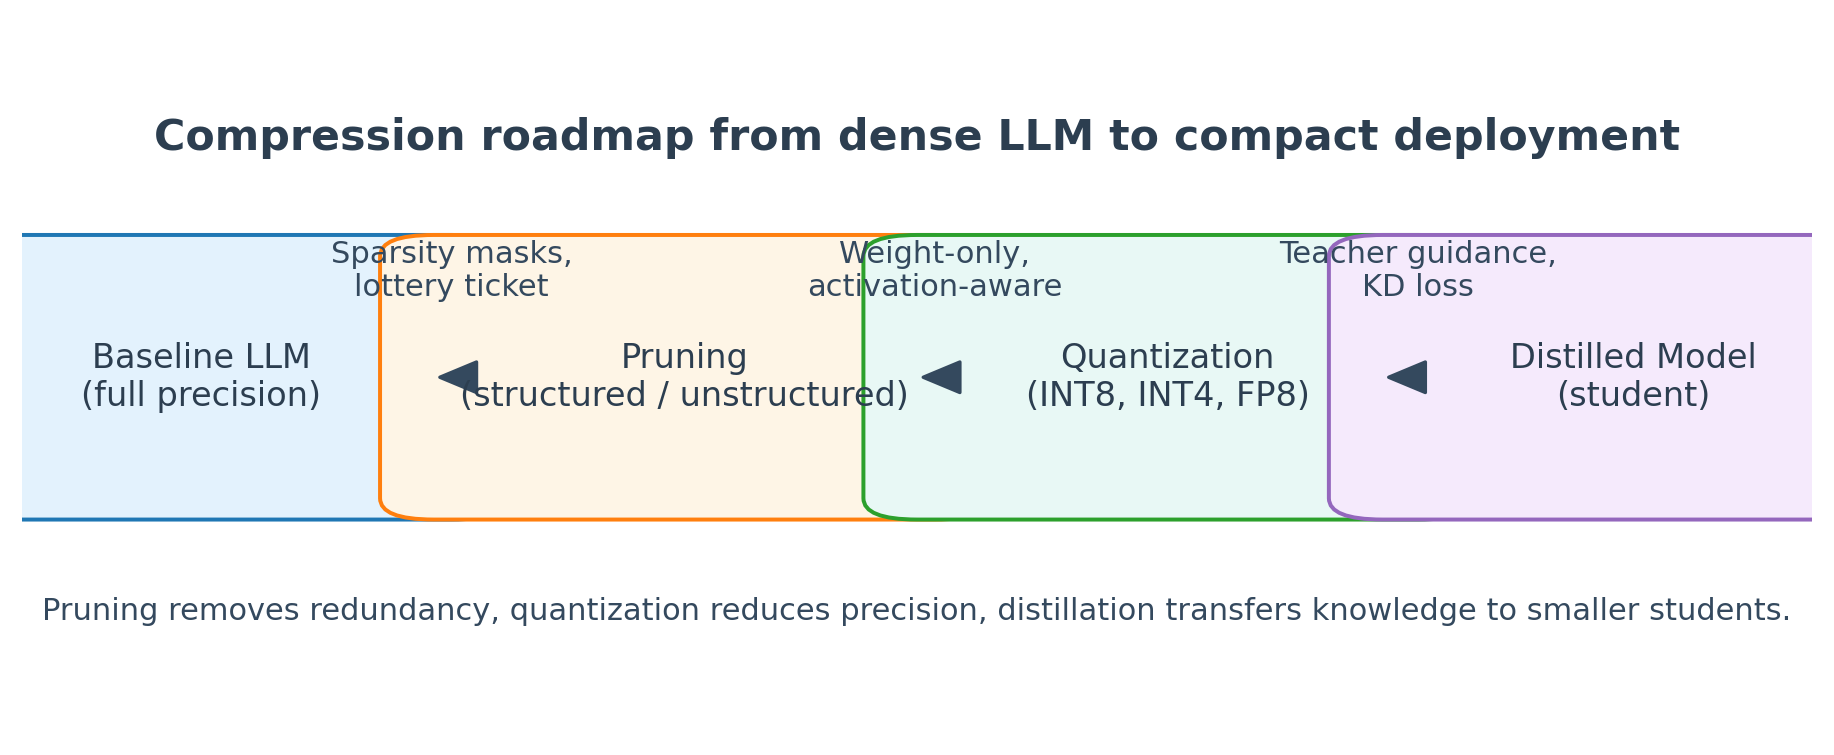
\includegraphics[width=0.9\textwidth]{compression_landscape.png}
  \caption{Compression roadmap combining pruning, quantization, and distillation.}
  \label{fig:compression_landscape_en}
\end{figure}

\subsection{Pruning strategies}
\begin{itemize}
  \item \textbf{Unstructured pruning:} Magnitude- or gradient-based removal of individual weights; flexible but hardware-unfriendly.
  \item \textbf{Structured pruning:} Drops entire channels, heads, or matrix columns, preserving dense matrix kernels.
  \item \textbf{Dynamic sparsity:} Methods like RigL or SNIP adjust sparsity masks during training for better convergence.
  \item \textbf{Lottery ticket subnetworks:} Identify sub-networks that can be retrained from scratch, guiding lightweight fine-tuning.
\end{itemize}

\subsection{Quantization taxonomy}
\begin{longtable}{p{3cm}p{3cm}p{4cm}p{4cm}}
\toprule
Method & Bit width & Highlights & Tooling \\
\midrule
Dynamic quantization & INT8 & On-the-fly activation stats during inference & PyTorch Dynamic Quantization \\
Static quantization & INT8 & Calibration dataset for scale/zero-point & TensorRT, ONNX Runtime \\
Weight-only quantization & INT4/INT3 & Compress weights while retaining FP16 activations & GPTQ, AWQ \\
Activation-aware quantization & INT8/INT4 & Jointly scales weights and activations & SmoothQuant, AQLM \\
Mixed precision & FP8/INT8 & Leverages modern accelerators (H100, Gaudi2) & TransformerEngine, DeepSpeed \\
\bottomrule
\end{longtable}

\subsection{GPTQ example}
\begin{lstlisting}[language=Python,caption={Applying GPTQ to quantize LLaMA weights}]
from auto_gptq import AutoGPTQForCausalLM, BaseQuantizeConfig
from transformers import AutoTokenizer

model_name = "meta-llama/Llama-2-7b-hf"
quant_config = BaseQuantizeConfig(bits=4, group_size=128, desc_act=False)

model = AutoGPTQForCausalLM.from_pretrained(model_name, quantize_config=quant_config)
tokenizer = AutoTokenizer.from_pretrained(model_name, use_fast=True)

model.quantize(
    examples=["Compression saves memory.", "GPTQ performs post-training quantization."],
    batch_size=8,
    use_triton=True,
)

model.save_quantized("llama2-7b-gptq")
tokenizer.save_pretrained("llama2-7b-gptq")
\end{lstlisting}

\section{Knowledge Distillation}
\subsection{Distillation workflow}
Knowledge distillation (KD) transfers inductive biases and behaviors from a teacher to a student:
\begin{itemize}
  \item \textbf{Soft targets:} Temperature-scaled logits guide the student via KL divergence.
  \item \textbf{Intermediate matching:} Align attention maps, hidden states, or gradients between teacher and student.
  \item \textbf{Task-specific KD:} Use teacher outputs on annotated or synthetic tasks to supervise student fine-tuning.
\end{itemize}

\subsection{Loss formulation}
\begin{equation}
\mathcal{L} = \alpha \mathcal{L}_{\text{KD}}(p_s, p_t) + \beta \mathcal{L}_{\text{task}}(y_s, y) + \gamma \mathcal{L}_{\text{feature}}(h_s, h_t),
\end{equation}
where $\alpha$, $\beta$, and $\gamma$ regulate the balance between soft targets, ground-truth labels, and feature alignment.

\subsection{Case highlights}
\begin{itemize}
  \item \textbf{TinyLlama:} 1.1B/3B students distilled from larger instruction-tuned teachers for mobile inference.
  \item \textbf{MiniLM:} Deep self-attention distillation yields compact BERT variants with competitive accuracy.
  \item \textbf{LLaDA:} Cross-lingual and multimodal knowledge distilled into smaller multilingual models.
\end{itemize}

\subsection{Teacher-student loop}
\begin{lstlisting}[language=Python,caption={Simplified knowledge distillation training loop}]
for batch in dataloader:
    with torch.no_grad():
        teach_out = teacher(**batch, output_hidden_states=True)

    stud_out = student(**batch, output_hidden_states=True)

    loss_kd = kl_divergence(
        F.log_softmax(stud_out.logits / T, dim=-1),
        F.softmax(teach_out.logits / T, dim=-1),
    ) * (T * T)

    loss_task = cross_entropy(stud_out.logits, batch["labels"])
    loss_hidden = mse_loss(
        stud_out.hidden_states[-1],
        projector(teach_out.hidden_states[-1]),
    )

    loss = alpha * loss_kd + beta * loss_task + gamma * loss_hidden
    loss.backward()
    optimizer.step()
    optimizer.zero_grad()
\end{lstlisting}

\section{TinyLLM and Edge Deployment}
\subsection{Deployment stack}
Figure~\ref{fig:tinyllm_edge_stack_en} illustrates the TinyLLM deployment stack: a compression pipeline generates compact models, a quantized runtime executes on heterogeneous hardware, and orchestration plus monitoring close the loop.
\begin{figure}[H]
  \centering
  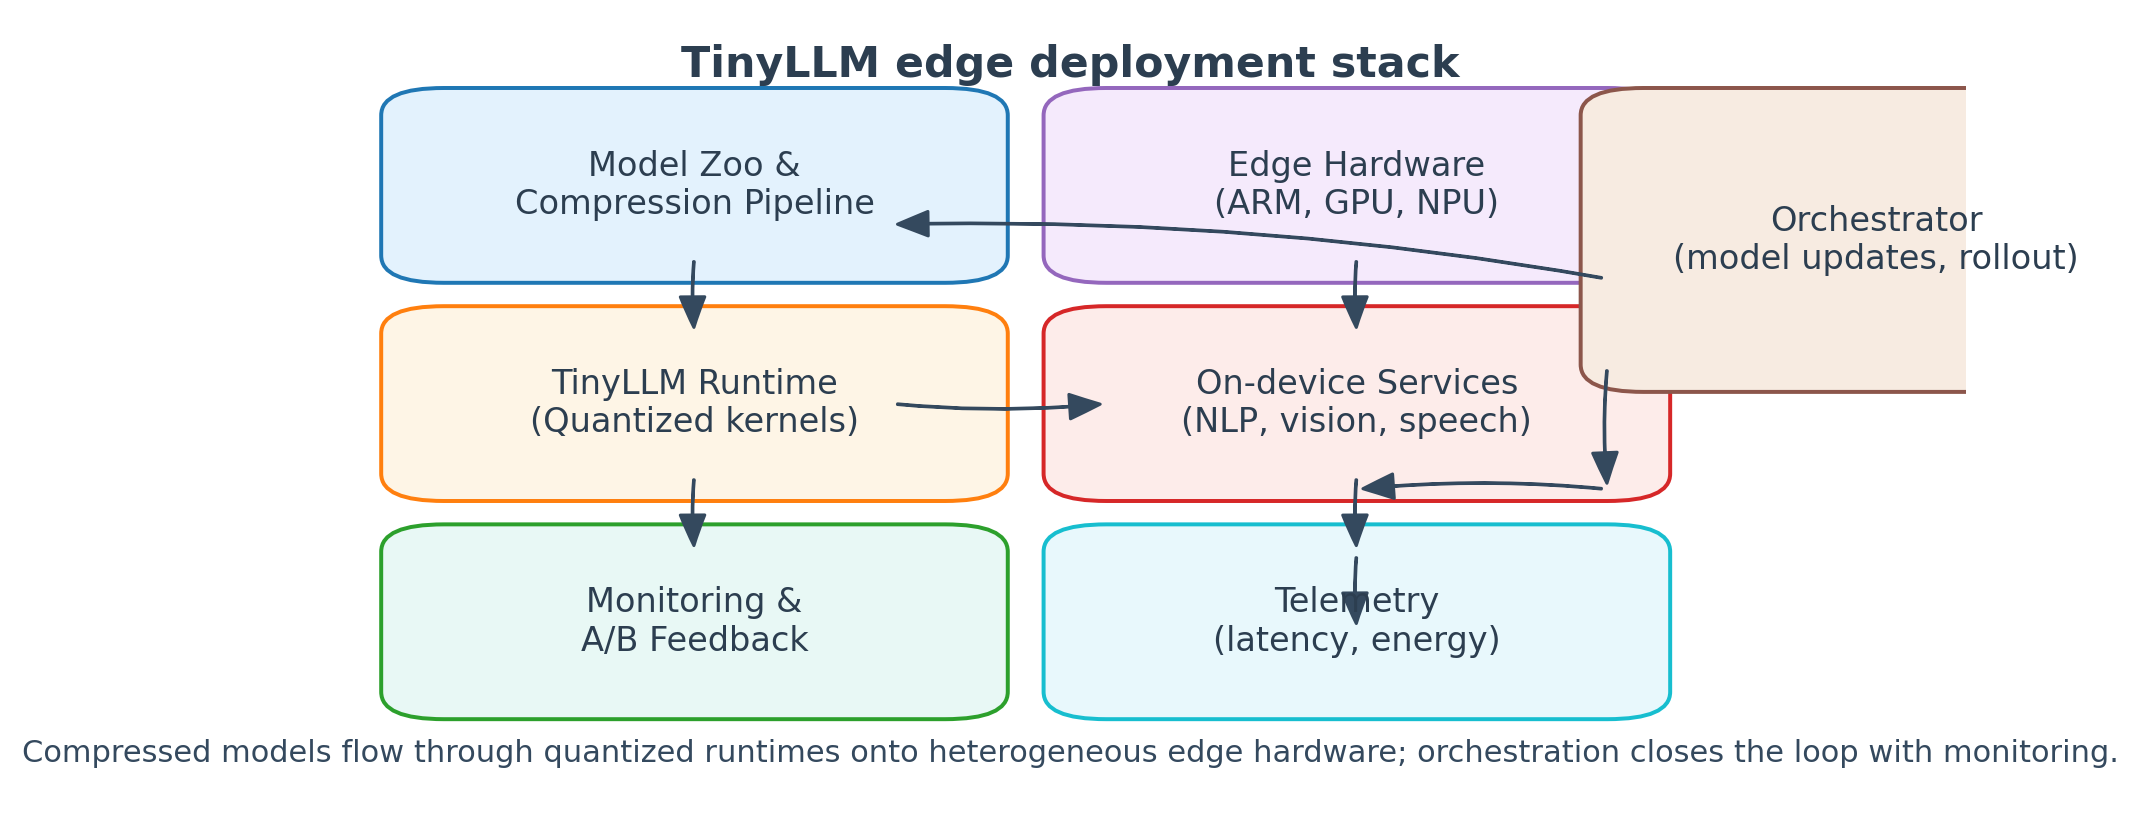
\includegraphics[width=0.9\textwidth]{tinyllm_edge_stack.png}
  \caption{TinyLLM edge deployment stack with compression pipeline, runtime, hardware, and governance.}
  \label{fig:tinyllm_edge_stack_en}
\end{figure}

\subsection{TinyLLM runtime features}
\begin{itemize}
  \item \textbf{Kernel optimization:} INT4/INT8 GEMMs, tensor slicing, pipelined attention, and paged KV caches.
  \item \textbf{Memory management:} Static pools, grouped-query attention, and streaming weights reduce footprint.
  \item \textbf{Scheduler:} Multi-tenant queueing, dynamic batching, latency-aware throttling for SLA compliance.
\end{itemize}

\subsection{Edge hardware matrix}
\begin{longtable}{p{3cm}p{3cm}p{4cm}p{4cm}}
\toprule
Hardware & Precision & Target workloads & Toolchain \\
\midrule
ARM CPUs (Neon) & INT8/INT4 & Offline assistants, smart speakers & MNN, NCNN, llama.cpp \\
NVIDIA Jetson & FP16/INT8 & Robotics, industrial inspection & TensorRT, FasterTransformer \\
Apple Neural Engine & 8-bit & On-device iOS assistants & Core ML, Metal Performance Shaders \\
Custom NPUs & INT4/INT2 & Automotive, smart home, wearables & ONNX Runtime EPs, Apache TVM \\
\bottomrule
\end{longtable}

\subsection{Deployment workflow}
\begin{enumerate}
  \item Compress base models via pruning + quantization + distillation into student checkpoints.
  \item Convert to target runtimes (ONNX, TensorRT, Core ML, GGUF).
  \item Integrate with TinyLLM or other inference runtimes (FasterTransformer, MNN, llama.cpp).
  \item Collect telemetry (latency, power, accuracy) and feed back into retraining or adaptive rollout.
\end{enumerate}

\subsection{Inference script}
\begin{lstlisting}[language=Python,caption={Running a quantized TinyLLM model with llama.cpp}]
import subprocess
from pathlib import Path

model_path = Path("models/tinyllm-q4_0.gguf")
prompt = "Provide a bilingual summary of today's incident reports."

cmd = [
    "./main",
    "-m", str(model_path),
    "-p", prompt,
    "-n", "160",
    "--temp", "0.7",
    "--batch-size", "48",
    "--threads", "6",
]

completed = subprocess.run(cmd, capture_output=True, text=True, check=True)
print(completed.stdout)
\end{lstlisting}

\section*{Operational recommendations}
\begin{itemize}
  \item Evaluate compression knobs jointly—quantization-aware pruning, sparse-aware distillation—to reach desired accuracy/fps goals.
  \item Establish regression suites covering perplexity, task accuracy, latency, and energy, plus red-team tests for safety.
  \item Instrument edge devices to gather anonymized telemetry; use data for continuous distillation and dynamic model selection.
  \item Harden edge deployments with encryption, secure boot, and policy enforcement despite local inference benefits.
\end{itemize}

\section*{Further reading}
\begin{itemize}
  \item Frantar et al. ``GPTQ: Accurate Post-Training Quantization for Generative Pre-trained Transformers.'' NeurIPS, 2022.
  \item Dettmers et al. ``QLoRA: Efficient Finetuning of Quantized LLMs.'' NeurIPS, 2023.
  \item Sanh et al. ``DistilBERT, a distilled version of BERT.'' NeurIPS, 2019.
  \item Zhang et al. ``TinyLlama: Tiny Language Models for Edge AI.'' arXiv, 2024.
  \item Li et al. ``AWQ: Activation-aware Weight Quantization for LLM Compression and Acceleration.'' arXiv, 2023.
\end{itemize}

\end{document}

